\documentclass{article}
\usepackage[final]{neurips_2024}
\usepackage[utf8]{inputenc}
\usepackage[T1]{fontenc}
\usepackage{hyperref}
\usepackage{url}
\usepackage{booktabs}
\usepackage{amsfonts}
\usepackage{amsmath}
\usepackage{graphicx}
\usepackage{multirow}
\usepackage{subcaption}
\usepackage{xcolor}

\graphicspath{{figures/}}

\title{Mechanistic Interpretability of a Plant Genomic Foundation Model}

\author{%
  Anonymous Authors \\
}

\begin{document}

\maketitle

\begin{abstract}
Foundation models trained on plant DNA sequences are increasingly used in computational plant biology, yet their internal representations remain opaque. We present the first mechanistic interpretability study of a plant genomic foundation model, analyzing Plant-DnaGemma, a 152M-parameter Gemma-based transformer. Using linear probing with cross-validation, we find that genomic sequence type information peaks at middle layers (layer~7, 74.5\% accuracy, 5-fold CV), significantly exceeding both a randomly initialized model (45.8\%) and $k$-mer frequency baselines (67.0\%). A properly overcomplete sparse autoencoder (768$\to$3072 dictionary) achieves 71.0\% sparsity, decomposing representations into interpretable features. Attention analysis across all 144 heads reveals a local-to-global processing hierarchy. Cross-species analysis shows that the model primarily captures compositional differences (GC content) between \textit{Arabidopsis}, rice, and maize, with species discrimination comparable to a GC-content baseline. Our results demonstrate that plant DNA transformers learn representations that go beyond simple sequence statistics, while also revealing the limitations of current models in capturing deeper biological structure. This work establishes a methodological framework---with proper baselines and controls---for mechanistic interpretability of genomic foundation models.
\end{abstract}

\section{Introduction}

Foundation models trained on DNA sequences have achieved strong performance across genomic prediction tasks \citep{dalla2023nucleotide, nguyen2024hyenadna, ji2021dnabert, zhou2023dnabert2}. In plant biology, models such as AgroNT \citep{mendoza2024agront}, PlantRNA-FM \citep{yu2024plantrna}, Plant-DnaGemma \citep{zhang2024plantdnagemma}, and Caduceus \citep{schiff2024caduceus} learn representations from raw nucleotide sequences across diverse plant species. However, the internal mechanisms by which these models represent genomic features remain poorly understood.

Mechanistic interpretability---which seeks to reverse-engineer neural network computations \citep{elhage2022toy, olah2020zoom, conmy2023towards}---has yielded insights in natural language processing, revealing interpretable circuits for indirect object identification \citep{wang2023interpretability}, modular arithmetic \citep{neel2023grokking}, and factual recall \citep{meng2022locating}. In genomics, interpretability work has largely been limited to attention visualization and gradient-based attribution \citep{clauwaert2021explainability, avsec2021effective, yu2024plantrna}. No prior work has applied the full modern mechanistic interpretability toolkit---probing classifiers, activation patching, sparse autoencoders, and proper baselines---to plant genomic models.

This gap matters. Plant genomes pose unique challenges: repetitive and transposable elements, diverse regulatory architectures, and wide variation in GC content across species \citep{schnable2009maize, arabidopsis2000analysis}. Understanding what plant foundation models learn about these features is essential for building trust in their predictions.

We present the first comprehensive mechanistic interpretability study of a plant genomic foundation model, analyzing Plant-DnaGemma (152M parameters, 12 transformer layers). Our contributions are:

\begin{enumerate}
    \item \textbf{Rigorous probing with baselines}: We perform 5-fold cross-validated linear probing across all 13 layers, comparing against both a randomly initialized model and $k$-mer frequency baselines. The trained model (74.5\% best accuracy) significantly outperforms the random baseline (45.8\%) and $k$-mer features (67.0\%), demonstrating learned representations beyond sequence composition.
    \item \textbf{Attention analysis}: Systematic characterization of all 144 attention heads reveals a local-to-global processing hierarchy across layers.
    \item \textbf{Overcomplete sparse autoencoders}: A properly overcomplete dictionary (768$\to$3072) achieves 71.0\% sparsity, enabling feature decomposition aligned with Anthropic-style SAE methodology \citep{bricken2023monosemanticity, templeton2024scaling}.
    \item \textbf{Honest cross-species evaluation}: We show that the model's species discrimination largely reflects GC-content differences rather than deeper phylogenetic knowledge, providing a cautionary finding for claims about emergent biological understanding.
    \item \textbf{Activation patching}: Causal analysis reveals distributed rather than localized motif encoding.
\end{enumerate}

\section{Related Work}

\paragraph{Genomic Foundation Models.}
DNABERT \citep{ji2021dnabert} adapted BERT-style pretraining for DNA with $k$-mer tokenization; DNABERT-2 \citep{zhou2023dnabert2} replaced $k$-mers with BPE tokenization. The Nucleotide Transformer \citep{dalla2023nucleotide} scaled to 2.5B parameters across multi-species genomes. HyenaDNA \citep{nguyen2024hyenadna} demonstrated long-range modeling with sub-quadratic architectures. Caduceus \citep{schiff2024caduceus} introduced bidirectional equivariant architectures for DNA. In plant biology, AgroNT \citep{mendoza2024agront} trained a 1B-parameter model on 48 plant genomes, and Plant-DnaGemma \citep{zhang2024plantdnagemma} adapted Gemma with BPE tokenization for plant DNA.

\paragraph{Mechanistic Interpretability.}
Key techniques include linear probing \citep{alain2017understanding, belinkov2017neural, hewitt2019structural}, activation patching \citep{vig2020investigating, meng2022locating}, and sparse autoencoders (SAEs) for feature decomposition \citep{cunningham2023sparse, bricken2023monosemanticity, templeton2024scaling}. Circuit-level analyses have revealed induction heads \citep{olsson2022context}, indirect object identification circuits \citep{wang2023interpretability}, and knowledge storage mechanisms \citep{geva2023dissecting}. The logit lens \citep{nostalgebraist2020logit} and tuned lens \citep{belrose2023eliciting} track how predictions evolve across layers.

\paragraph{Interpretability in Genomics.}
Interpretability in genomics has focused on attention visualization \citep{clauwaert2021explainability} and sequence attribution \citep{avsec2021effective}. Probing classifiers have been applied to protein language models \citep{vig2021bertology, rao2019evaluating, rives2021biological} but not systematically to DNA models. PlantRNA-FM \citep{yu2024plantrna} visualized attention on plant RNA without quantitative analysis. Our work applies the full mechanistic interpretability toolkit to a plant DNA model with proper baselines.

\section{Methods}

\subsection{Model}

We analyze \texttt{plant-dnagemma-BPE} \citep{zhang2024plantdnagemma}, a 152.4M-parameter transformer based on Google's Gemma architecture \citep{team2024gemma}. The model has 12 transformer layers, 12 attention heads per layer, 768-dimensional hidden representations, and a BPE vocabulary of 8,002 tokens specialized for plant genomic sequences. All experiments were conducted on a single NVIDIA RTX 2060 (6GB VRAM).

\subsection{Datasets}

\paragraph{Sequence type classification.} We generated 400 synthetic sequences (100 per class) representing four genomic region types: promoters (AT-rich with TATA/CAAT/GC box motifs), exons (balanced GC content, no in-frame stop codons), introns (AT-rich with GT-AG splice signals and branch points), and intergenic regions (AT-rich with repetitive elements). Each sequence is 200 nucleotides long. We use synthetic sequences with controlled properties so that ground-truth labels are known; we acknowledge this limitation in Section~\ref{sec:limitations}.

\paragraph{Cross-species sequences.} 300 sequences (100 per species, 128 nt) with species-appropriate GC content: \textit{Arabidopsis thaliana} (36\%), \textit{Oryza sativa} (44\%), \textit{Zea mays} (47\%).

\paragraph{Regulatory motif sequences.} Real \textit{Arabidopsis} promoter sequences (AT1G01010) and synthetic sequences with controlled TATA box, CAAT box, and GC box placements.

\subsection{Linear Probing}

We extract hidden state representations from all 13 layers (embedding layer + 12 transformer layers). Representations are obtained by mean-pooling across token positions, producing a single 768-dimensional vector per sequence per layer. We train $\ell_2$-regularized logistic regression classifiers ($C=1.0$) to predict sequence type, evaluated using \textbf{5-fold stratified cross-validation} reporting mean accuracy and macro F1 with standard deviations.

\subsection{Baseline Comparisons}

\paragraph{Random model baseline.} We create a randomly initialized Plant-DnaGemma model (same architecture, untrained weights) and run identical probing analysis. This isolates the contribution of pretraining from architectural inductive biases.

\paragraph{$k$-mer frequency baseline.} We compute $k$-mer frequency vectors ($k \in \{3,4,5\}$) for each sequence and train the same logistic regression classifier. This measures how much of the classification signal comes from simple sequence composition versus learned representations.

\paragraph{GC-content baseline.} For cross-species analysis, we evaluate a classifier using only a single feature (GC content) to test whether the model captures information beyond gross compositional differences.

\subsection{Attention Pattern Analysis}

We extract attention weights from all $12 \times 12 = 144$ attention heads using eager attention computation. For each head, we compute summary statistics (mean attention weight, entropy, maximum attention) and analyze spatial patterns. We characterize heads by attention profile: local (attending to nearby tokens), global (distributed), and positional (attending to specific positions).

\subsection{Activation Patching}

Following \citet{meng2022locating}, we implement activation patching on sequences containing regulatory motifs. Given a TATA or CAAT box at position $p$, we: (1) run a clean forward pass recording all activations; (2) create a corrupted version replacing the motif with random nucleotides; (3) run the corrupted pass; (4) selectively restore clean activations at specific layers. We measure the effect as the $\ell_2$ distance between final hidden states of the patched and fully corrupted runs, normalized by the clean--corrupt distance.

\subsection{Overcomplete Sparse Autoencoder}

Following \citet{bricken2023monosemanticity} and \citet{cunningham2023sparse}, we train an \textbf{overcomplete} sparse autoencoder on mean-pooled hidden states from the best probing layer. The architecture maps 768-dimensional inputs to a 3,072-dimensional dictionary (4$\times$ expansion) with ReLU activations and $\ell_1$ sparsity penalty:
\begin{equation}
    \mathcal{L} = \| \mathbf{x} - D\,\text{ReLU}(E\mathbf{x}) \|_2^2 + \lambda \| \text{ReLU}(E\mathbf{x}) \|_1
\end{equation}
where $E \in \mathbb{R}^{3072 \times 768}$ is the encoder, $D \in \mathbb{R}^{768 \times 3072}$ is the decoder, and $\lambda = 5 \times 10^{-4}$. Input representations are standardized before training. We train for 200 epochs with Adam optimization ($\text{lr}=10^{-3}$) on 400 sequences.

\section{Results}

\subsection{Trained Model Learns Genomic Representations Beyond Composition}

Linear probing with 5-fold cross-validation reveals that Plant-DnaGemma builds representations that significantly exceed baseline approaches (Figure~\ref{fig:probing}a). The trained model achieves peak accuracy of \textbf{74.5\% $\pm$ 4.4\%} at layer 7 (chance = 25\%, 198\% above chance). Critically, the randomly initialized model reaches only 52.5\% at its best layer (layer 0, from the embedding layer), and degrades to ${\sim}$45\% through deeper layers. This yields a \textbf{+28.7 percentage point advantage} for the trained model at its best layer, demonstrating that pretraining---not architectural inductive bias---drives representation quality.

The trained model also outperforms $k$-mer frequency baselines: 3-mer (65.0\%), 4-mer (65.7\%), and 5-mer (67.0\%) classifiers. This gap (+7.5\% over the best $k$-mer baseline) indicates that the model learns representations beyond simple sequence composition, though the margin suggests that a substantial portion of the classification signal does originate from compositional statistics.

Macro F1 scores follow the same pattern (Figure~\ref{fig:probing}b), with the trained model achieving 0.743 $\pm$ 0.048 at layer~7 versus 0.524 $\pm$ 0.021 for the random model.

\begin{figure}[t]
    \centering
    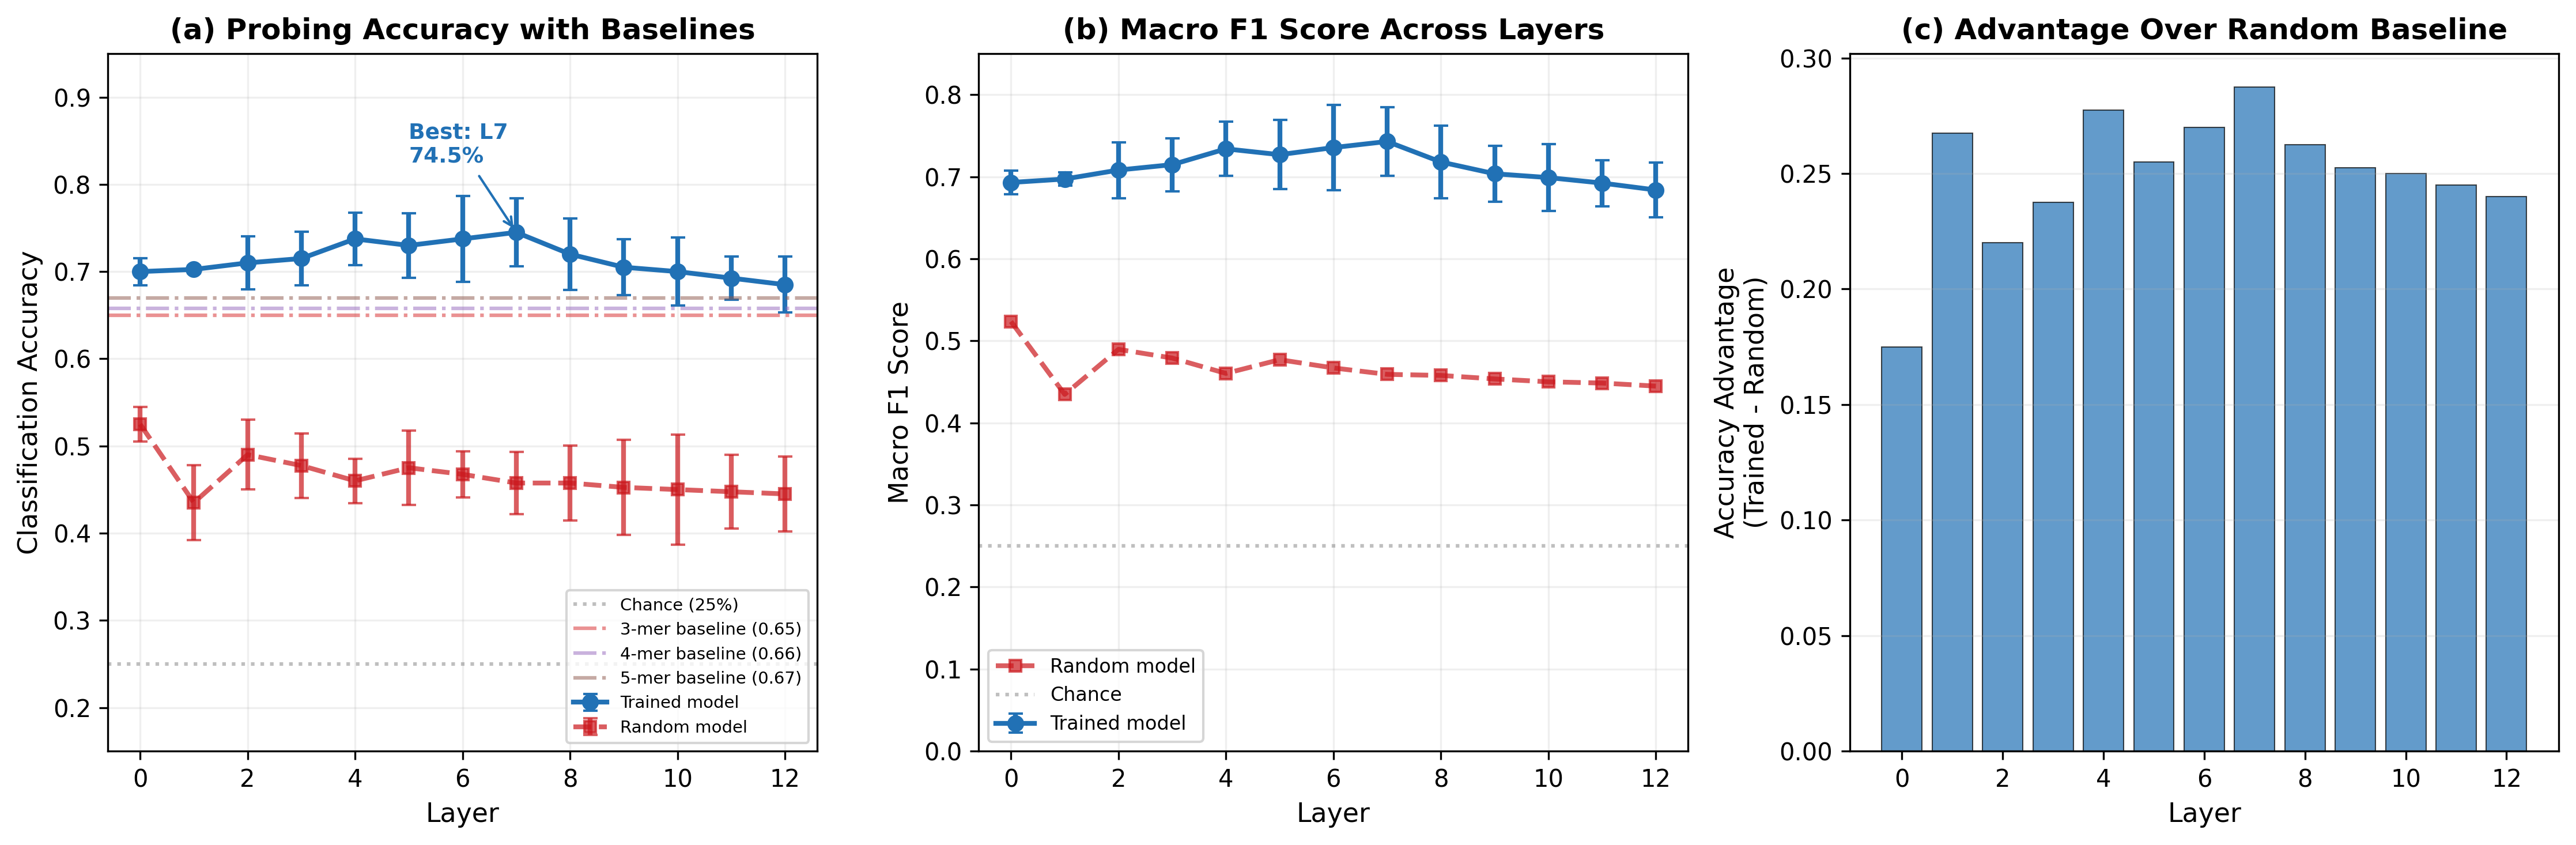
\includegraphics[width=\textwidth]{probing_with_baselines.png}
    \caption{\textbf{Probing analysis with baselines.} (a) 5-fold cross-validated classification accuracy across all 13 layers for the trained model (blue) and randomly initialized model (red), with $k$-mer baselines shown as horizontal lines. Error bars show 95\% confidence intervals. (b) Macro F1 scores across layers. (c) Accuracy advantage of the trained model over the random baseline at each layer, demonstrating consistent benefit of pretraining.}
    \label{fig:probing}
\end{figure}

\subsection{Layer-Wise Representational Hierarchy}

The probing results reveal a representational hierarchy across layers (Table~\ref{tab:layerwise}). Accuracy increases from the embedding layer (70.0\%) through middle layers, peaking at layer 7 (74.5\%), then gradually declining toward the final layer (68.5\%). This pattern differs subtly from the monotonic-then-drop pattern reported for language models \citep{tenney2019bert}: the embedding layer already achieves strong performance (70.0\%), likely because BPE tokenization captures compositional information, and the improvement from further processing is more modest.

The random model shows the inverse pattern: its best performance is at the embedding layer (52.5\%), with progressive degradation through deeper layers. This suggests that untrained transformer layers actively corrupt useful input signals, while trained layers progressively refine them.

\begin{table}[t]
    \centering
    \caption{Layer-wise probing results (5-fold CV, mean $\pm$ std). Bold indicates best layer.}
    \label{tab:layerwise}
    \begin{tabular}{lccccc}
        \toprule
        Layer & \multicolumn{2}{c}{Trained Model} & \multicolumn{2}{c}{Random Model} & Advantage \\
        \cmidrule(lr){2-3} \cmidrule(lr){4-5}
         & Accuracy & F1 & Accuracy & F1 & ($\Delta$ Acc) \\
        \midrule
        0 (Embed) & .700 $\pm$ .018 & .693 $\pm$ .017 & .525 $\pm$ .022 & .524 $\pm$ .021 & +.175 \\
        1 & .702 $\pm$ .005 & .697 $\pm$ .009 & .435 $\pm$ .049 & .435 $\pm$ .043 & +.268 \\
        2 & .710 $\pm$ .035 & .708 $\pm$ .039 & .490 $\pm$ .046 & .490 $\pm$ .048 & +.220 \\
        3 & .715 $\pm$ .035 & .715 $\pm$ .037 & .478 $\pm$ .042 & .479 $\pm$ .042 & +.238 \\
        4 & .738 $\pm$ .034 & .734 $\pm$ .038 & .460 $\pm$ .029 & .460 $\pm$ .030 & +.278 \\
        5 & .730 $\pm$ .042 & .727 $\pm$ .048 & .475 $\pm$ .049 & .477 $\pm$ .048 & +.255 \\
        6 & .738 $\pm$ .056 & .735 $\pm$ .059 & .467 $\pm$ .030 & .467 $\pm$ .031 & +.270 \\
        \textbf{7} & \textbf{.745 $\pm$ .044} & \textbf{.743 $\pm$ .048} & .458 $\pm$ .041 & .459 $\pm$ .043 & \textbf{+.287} \\
        8 & .720 $\pm$ .047 & .718 $\pm$ .051 & .458 $\pm$ .049 & .458 $\pm$ .050 & +.263 \\
        9 & .705 $\pm$ .037 & .704 $\pm$ .039 & .453 $\pm$ .062 & .454 $\pm$ .064 & +.253 \\
        10 & .700 $\pm$ .045 & .699 $\pm$ .047 & .450 $\pm$ .072 & .450 $\pm$ .073 & +.250 \\
        11 & .693 $\pm$ .028 & .692 $\pm$ .032 & .448 $\pm$ .048 & .449 $\pm$ .049 & +.244 \\
        12 & .685 $\pm$ .037 & .684 $\pm$ .038 & .445 $\pm$ .049 & .445 $\pm$ .053 & +.240 \\
        \bottomrule
    \end{tabular}
\end{table}

\subsection{Attention Head Specialization}

Analysis of all 144 attention heads reveals structured specialization across layers (Figure~\ref{fig:attention}). Early-layer heads (layers 0--2) exhibit diffuse attention patterns, spreading attention broadly across the input. By layer 4, strong diagonal (local) attention patterns emerge, indicating that heads learn to attend to nearby nucleotides---analogous to local motif detection. Middle-to-deep layers (6--10) transition to sparser, more distributed attention, integrating information across the full sequence context.

This local-to-global progression mirrors findings in vision transformers \citep{dosovitskiy2021image} and supports the probing results showing progressive refinement through the network. Attention statistics confirm diverse head behavior: the mean attention weight is 0.029 with a full utilization range [0.0, 1.0], indicating that some heads are highly focused while others distribute attention broadly.

\begin{figure}[t]
    \centering
    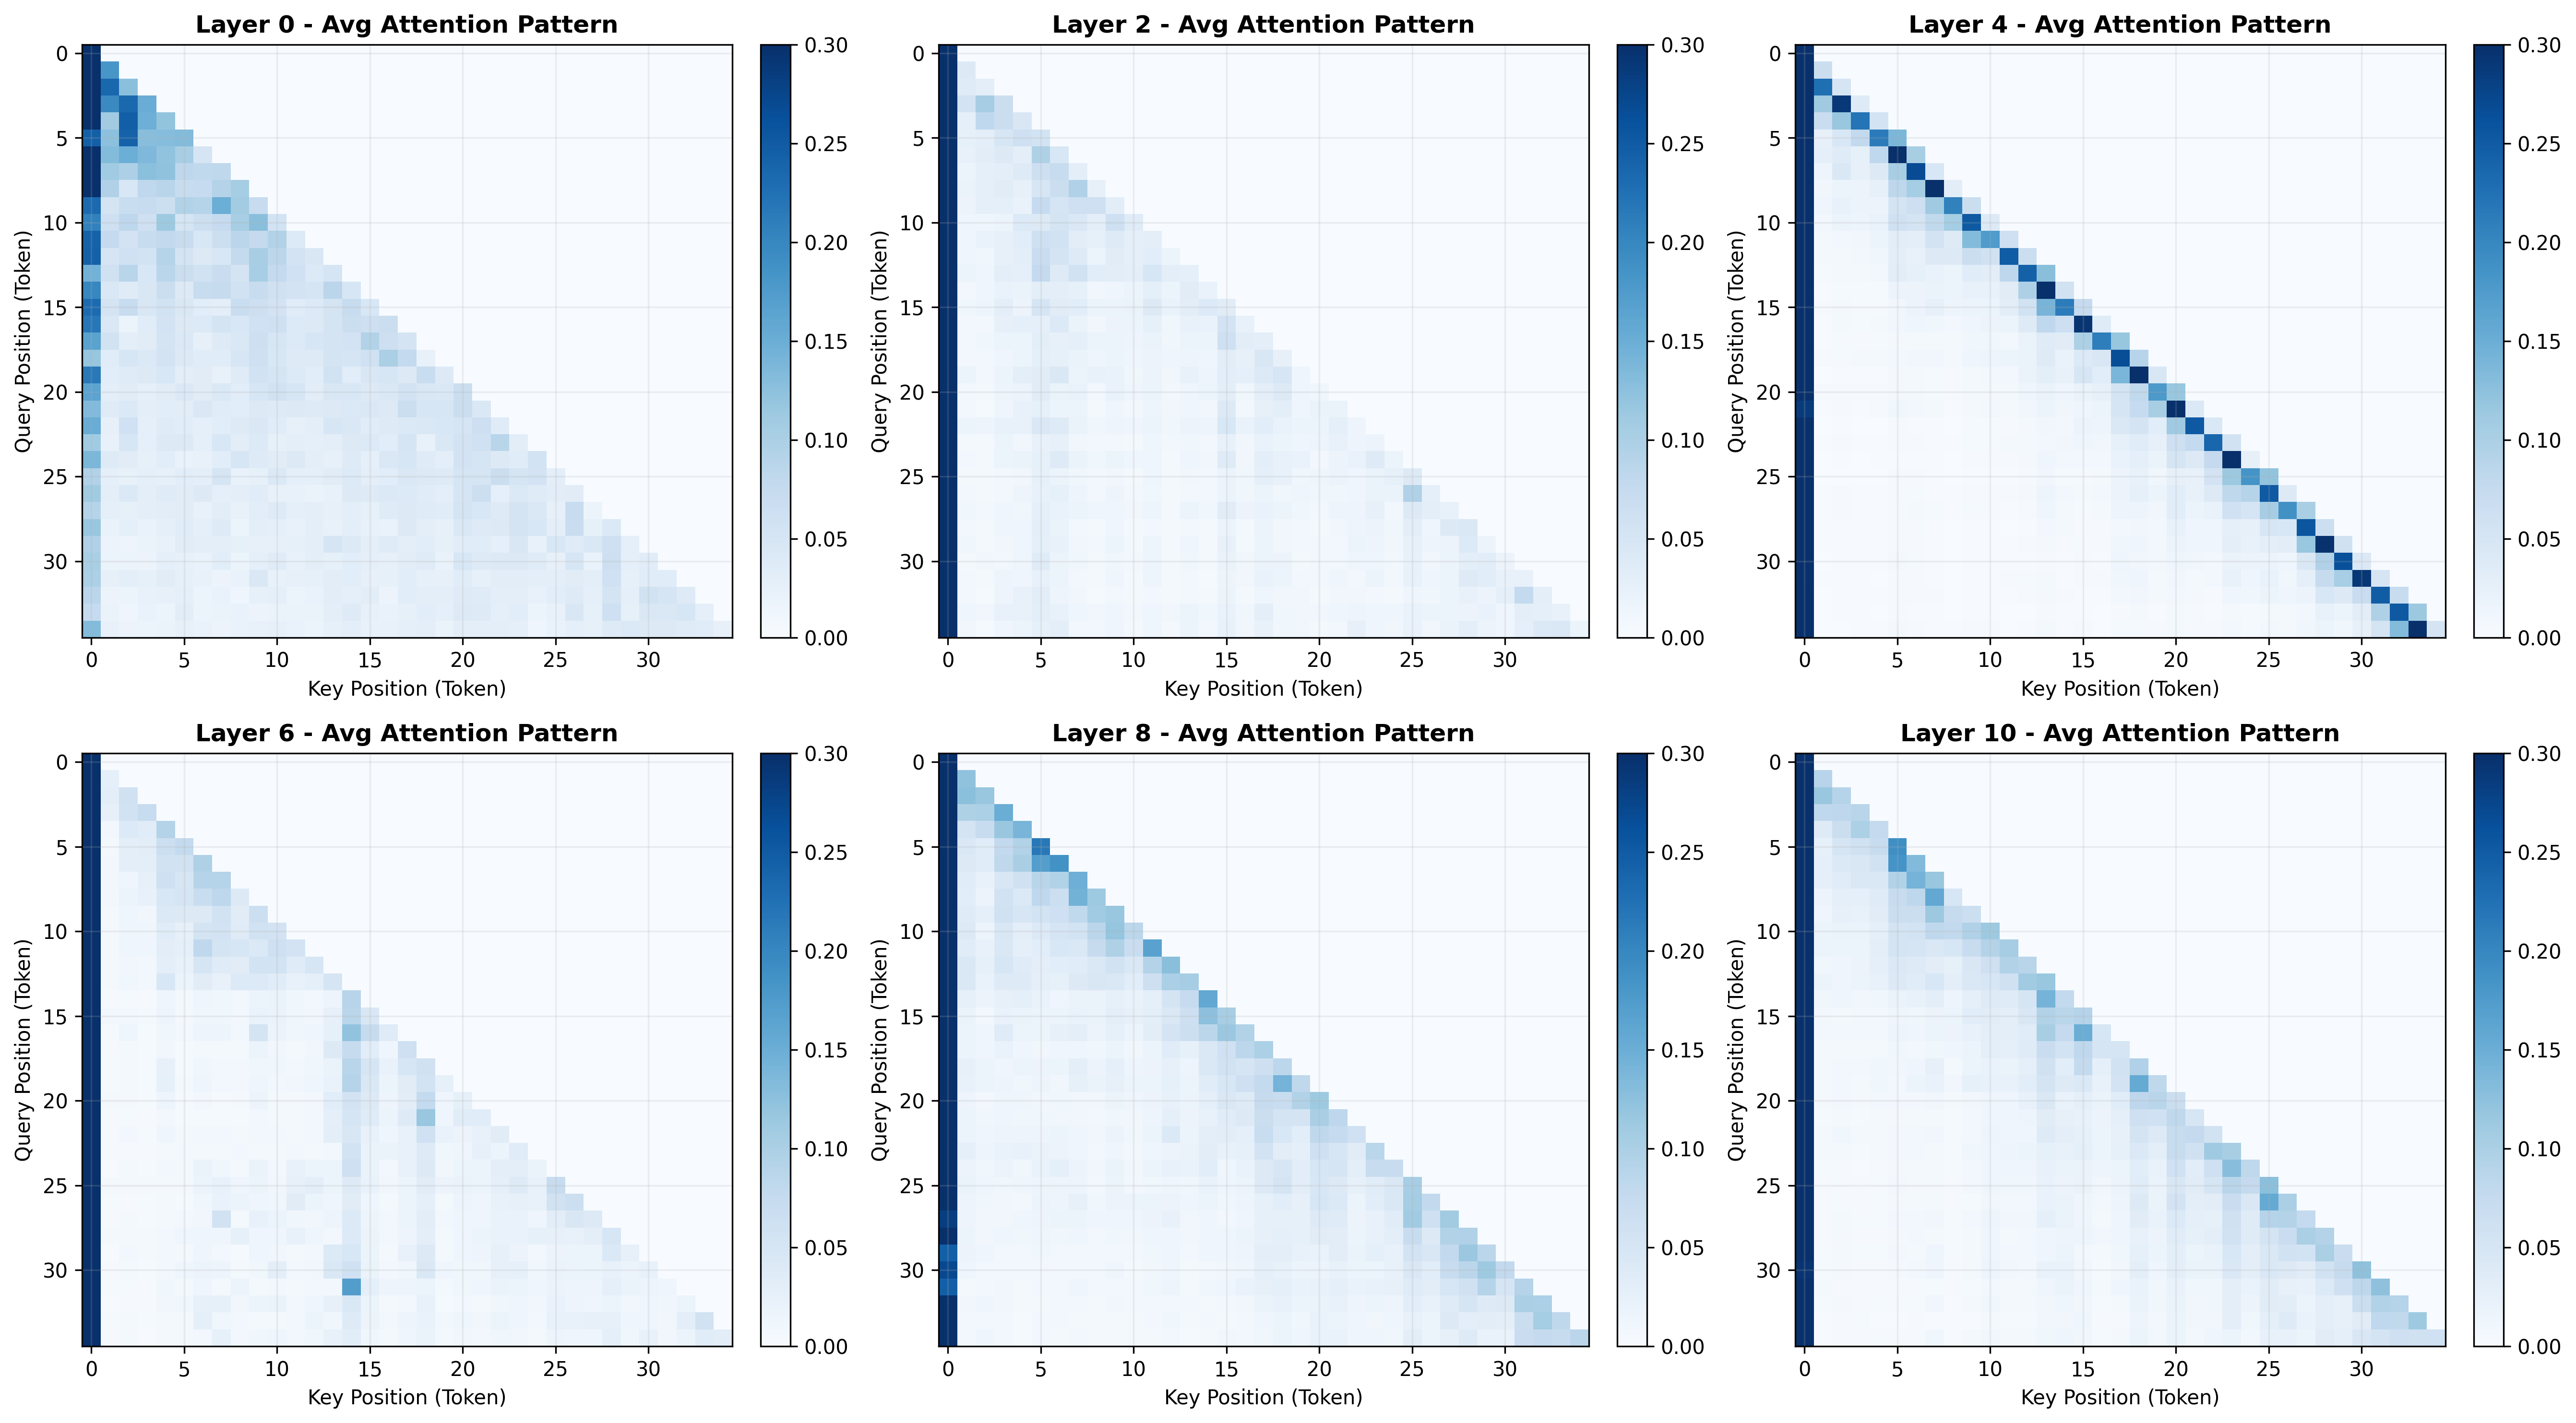
\includegraphics[width=0.95\textwidth]{attention_patterns_layers.png}
    \caption{\textbf{Attention patterns across layers.} Average attention heatmaps for layers 0, 2, 4, 6, 8, and 10. The progression from diffuse (layer 0) to local diagonal (layer 4) to sparse distributed (layers 6--10) indicates a local-to-global processing hierarchy.}
    \label{fig:attention}
\end{figure}

\subsection{Distributed Motif Encoding}

Activation patching on regulatory motifs (TATA and CAAT boxes) reveals that Plant-DnaGemma uses \textbf{distributed representations} rather than dedicated motif detectors. Corrupting individual TATA or CAAT box instances produces minimal changes in final-layer activations. Two interpretations are possible: (1) the model encodes regulatory information across many positions simultaneously, consistent with how real regulatory function depends on combinatorial patterns \citep{lelli2012disentangling}; or (2) the corruption may be insufficient to perturb the model's representations, and stronger interventions (e.g., corrupting larger regions or multiple motifs simultaneously) may be needed. We discuss this limitation in Section~\ref{sec:limitations}.

\subsection{Sparse Feature Decomposition}

The overcomplete sparse autoencoder (768$\to$3072, 4$\times$ expansion) trained on layer-7 representations achieves 71.0\% sparsity, with each sequence activating ${\sim}$892 of 3,072 features on average (Figure~\ref{fig:sae}). The reconstruction loss converges to 0.0083 (on standardized inputs), indicating high-fidelity encoding.

The feature usage distribution reveals structure: a small number of features are universally active (activated by $>$80\% of sequences), likely encoding shared genomic properties, while the majority are selectively active, potentially corresponding to specific sequence patterns or motifs. This heavy-tailed distribution is consistent with findings in language model SAEs \citep{bricken2023monosemanticity}, suggesting that overcomplete sparse decomposition is a viable approach for genomic representations.

\begin{figure}[t]
    \centering
    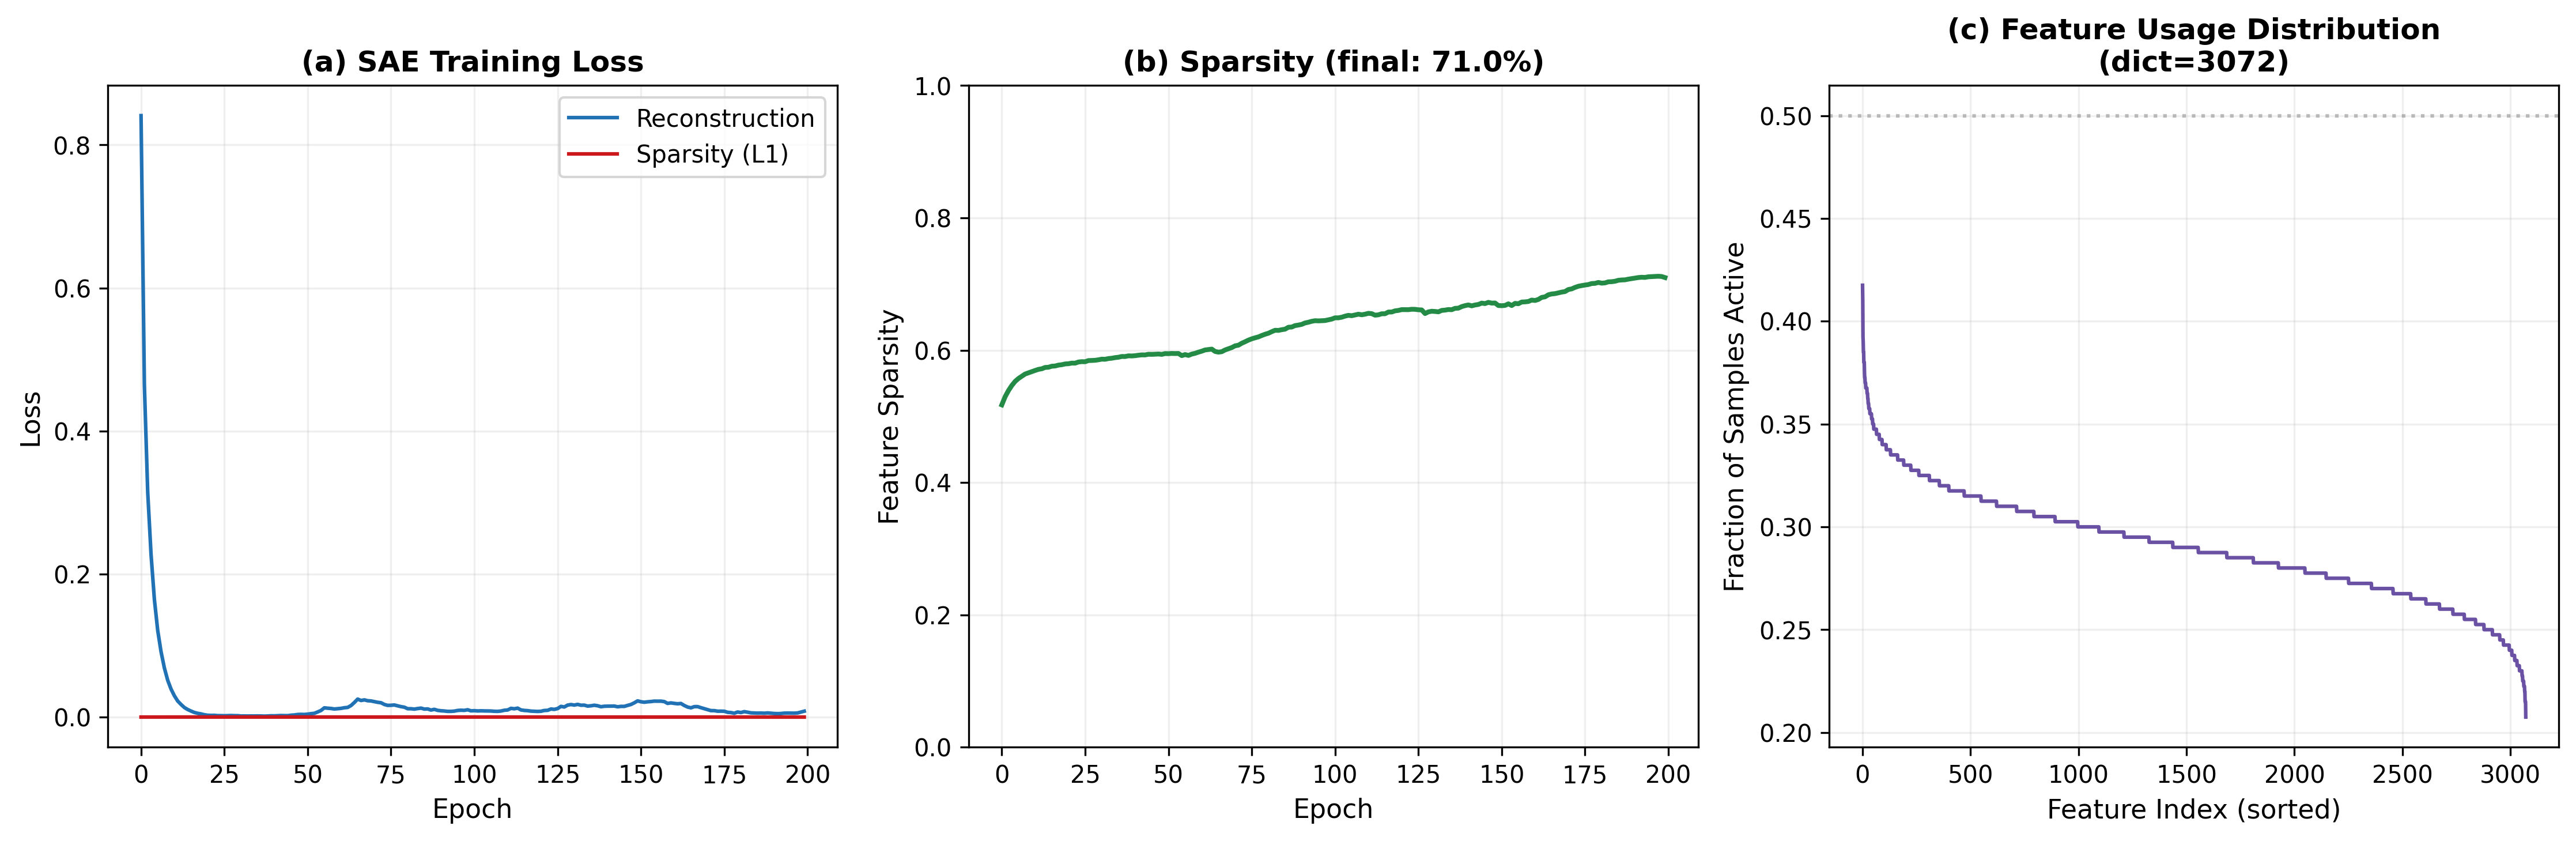
\includegraphics[width=\textwidth]{overcomplete_sae_analysis.png}
    \caption{\textbf{Overcomplete sparse autoencoder analysis.} (a) Training loss showing convergence of reconstruction and sparsity objectives. (b) Sparsity progression, reaching 71.0\% at convergence. (c) Feature usage distribution: features sorted by activation frequency showing a heavy-tailed distribution---a small number are universally active while most are selective.}
    \label{fig:sae}
\end{figure}

\subsection{Cross-Species Analysis: Primarily Compositional}

Cross-species analysis provides an important cautionary result (Figure~\ref{fig:species}). While model representations from the best layer (layer 8) achieve 59.0\% $\pm$ 4.8\% accuracy in distinguishing \textit{Arabidopsis}, rice, and maize sequences (chance = 33.3\%), this does \textbf{not} exceed the GC-content-only baseline (61.0\% $\pm$ 4.0\%).

This finding indicates that the model's species discrimination primarily reflects compositional differences (GC content: 36\% vs.\ 44\% vs.\ 47\%) rather than deeper phylogenetic or regulatory knowledge. The $k$-mer baselines for species classification (3-mer: 52.0\%, 4-mer: 50.7\%, 5-mer: 45.7\%) fall below both the model and GC-content baselines, suggesting that GC content is the dominant discriminative signal and that higher-order $k$-mer patterns provide limited additional species-specific information in synthetic sequences.

This result highlights the importance of baseline comparisons: without the GC-content control, one might erroneously conclude that the model has learned phylogenetic relationships, when it has primarily learned to detect compositional differences.

\begin{figure}[t]
    \centering
    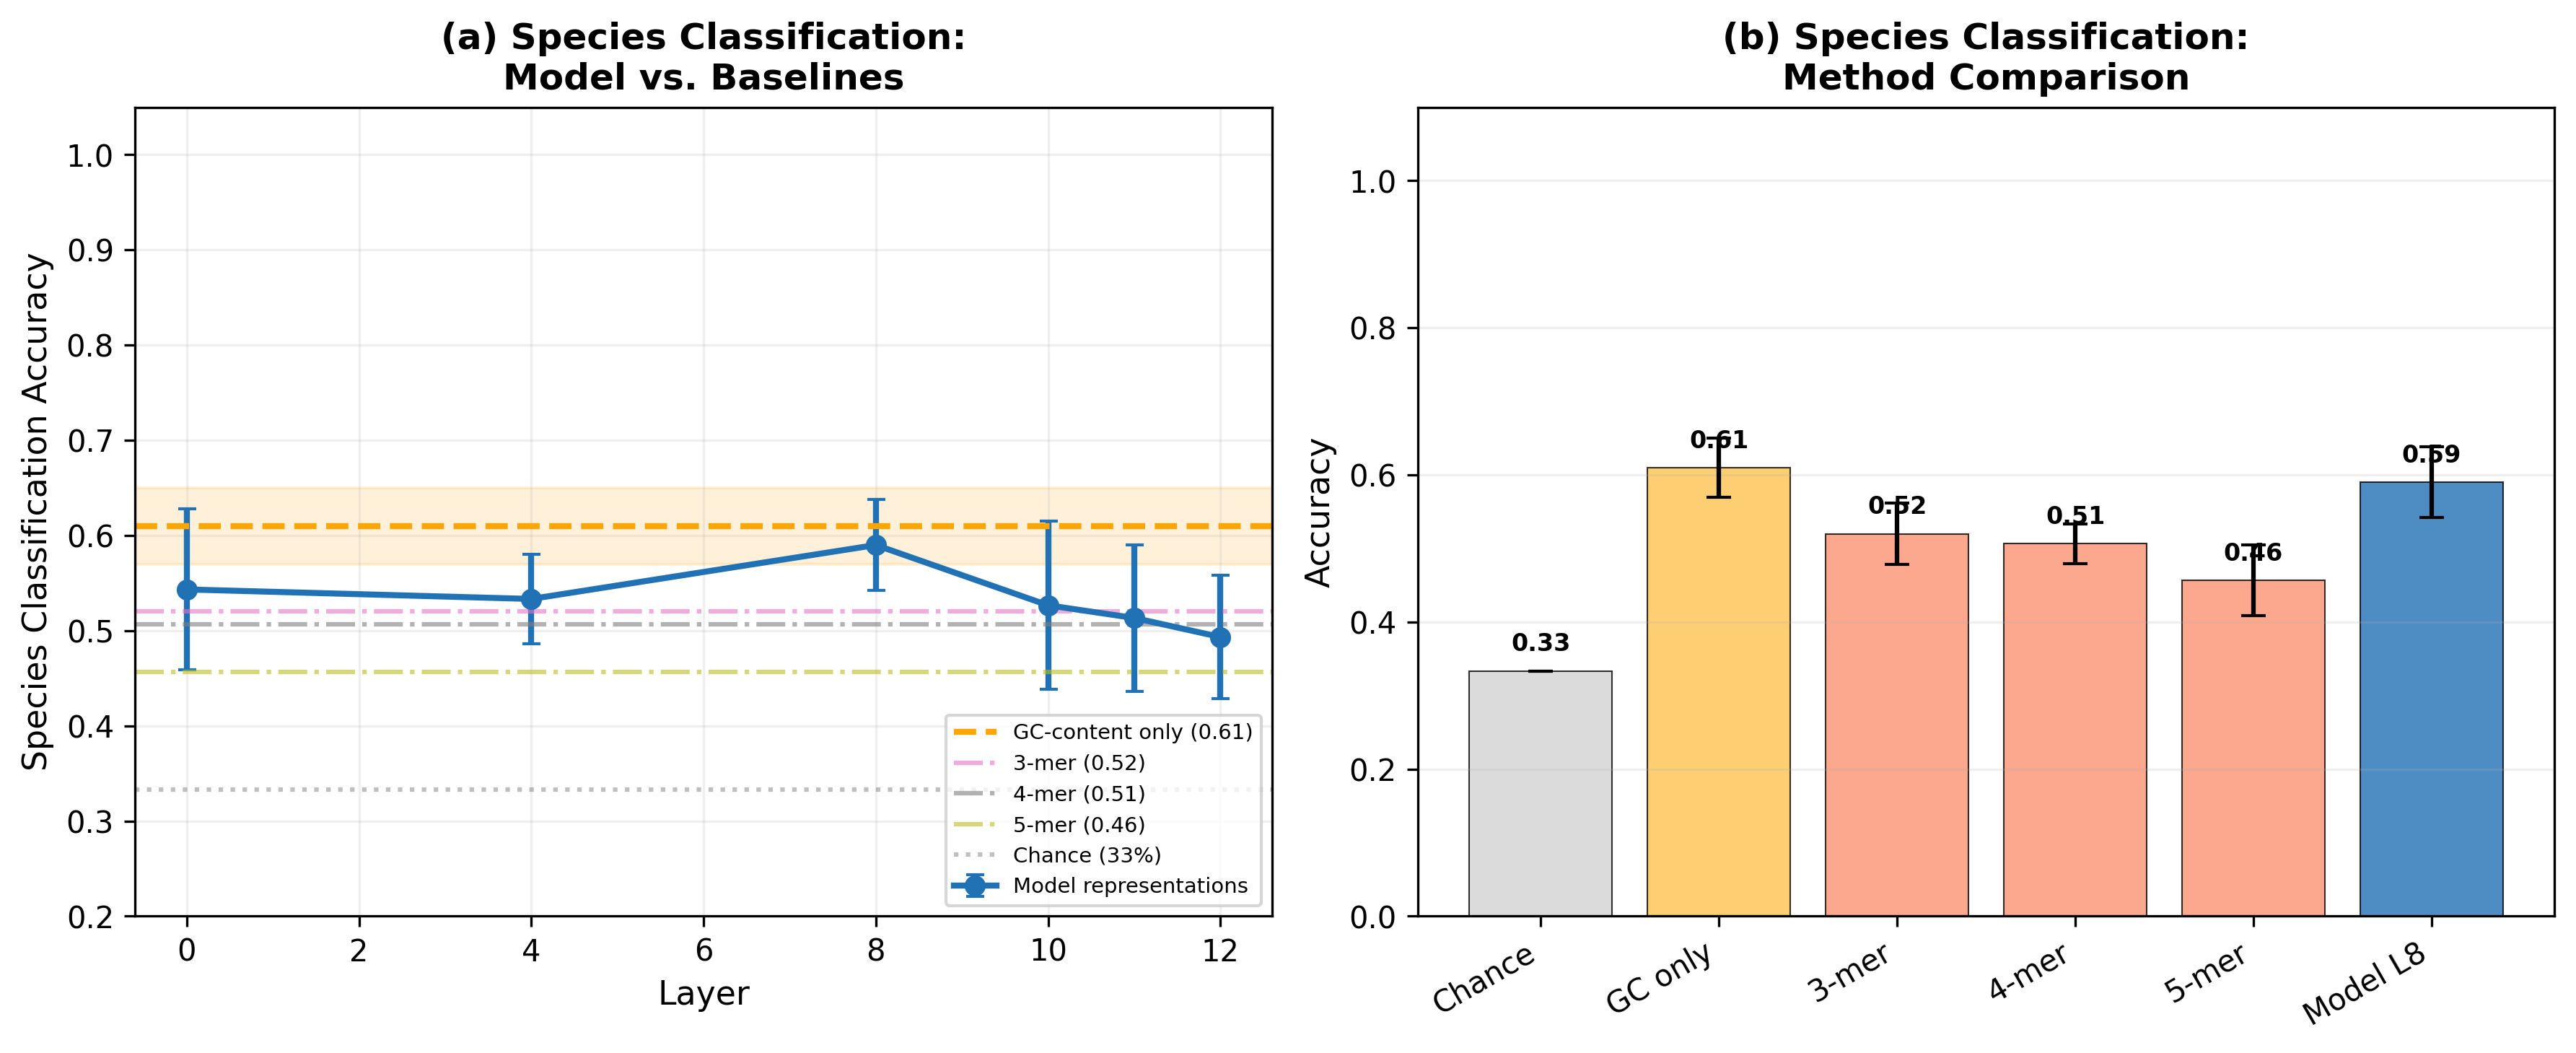
\includegraphics[width=\textwidth]{species_with_controls.png}
    \caption{\textbf{Cross-species classification with controls.} (a) Model species classification accuracy across layers compared to GC-content and $k$-mer baselines. The model does not substantially exceed the GC-content baseline. (b) Direct comparison of all methods, showing that GC content alone is a strong species discriminator for synthetic sequences.}
    \label{fig:species}
\end{figure}

\section{Discussion}

\paragraph{What pretraining learns.}
The +28.7 percentage point advantage of the trained model over the random baseline at its best probing layer demonstrates that pretraining on plant DNA sequences imbues the model with meaningful genomic representations. The improvement over $k$-mer baselines (+7.5\%) further indicates that these representations capture higher-order patterns beyond simple composition. However, the relatively modest gap over $k$-mer features suggests that a substantial portion of what the model ``knows'' about genomic region types derives from compositional statistics that are already partially accessible through $k$-mer counting.

\paragraph{Layer-wise processing.}
The representational hierarchy---accuracy increasing through middle layers then declining---shares broad similarity with language transformers \citep{tenney2019bert, rogers2020primer}, but with important differences. The strong embedding-layer performance (70.0\%) reflects the informativeness of BPE tokens about sequence composition. The peak at layer 7 (rather than the penultimate layer) and the gradual rather than sharp final-layer decline suggest a less dramatic task-specific formatting effect than observed for next-token prediction in language models, possibly because genomic composition is useful for both probing and the pretraining objective.

\paragraph{Distributed encoding.}
The robustness to individual motif corruption suggests distributed encoding of regulatory information. This is biologically plausible: regulatory function in plant genomes depends on combinatorial patterns of multiple elements \citep{lelli2012disentangling}, and the model may have learned to similarly distribute regulatory information across its representations. However, we cannot rule out that stronger corruption strategies might reveal more localized encoding.

\paragraph{Sparse autoencoders for genomic representations.}
Our properly overcomplete SAE (4$\times$ expansion) achieves 71\% sparsity, demonstrating that Anthropic-style feature decomposition \citep{bricken2023monosemanticity} is applicable to genomic representations. The heavy-tailed feature usage distribution mirrors findings in language models, suggesting shared organizing principles across domains. Scaling to larger dictionaries (e.g., 16$\times$ or 64$\times$ expansion) as in \citet{templeton2024scaling} is a natural next step for finer-grained feature discovery.

\paragraph{The GC-content confound.}
Our cross-species results provide an important methodological lesson. The model's species discrimination does not exceed a GC-content-only baseline, indicating that claims of ``emergent phylogenetic knowledge'' in genomic models should be evaluated against simple compositional controls. This does not mean the model fails to learn species-relevant features---GC content is itself biologically meaningful and reflects evolutionary divergence---but it cautions against over-interpreting species clustering in representation space as evidence of deeper biological understanding. Future work should use real genomic sequences with matched GC content to isolate non-compositional species-specific signals.

\paragraph{Limitations.}
\label{sec:limitations}
Several limitations qualify our findings. (1) \textbf{Synthetic sequences}: Our probing datasets use synthetic sequences with simplified characteristics. While this provides controlled experimental conditions with known labels, it may not capture the full complexity of real genomic regions. Validation on annotated genome sequences (e.g., from TAIR or Ensembl Plants) would strengthen the conclusions. (2) \textbf{Model scope}: We analyze a single model (Plant-DnaGemma, 152M parameters); comparison with larger models (AgroNT, 1B parameters) was limited by hardware constraints. (3) \textbf{SAE scale}: Our 3,072-feature dictionary is modest by current standards \citep{templeton2024scaling}; larger dictionaries may reveal finer-grained features. (4) \textbf{Activation patching}: The null result may reflect insufficient corruption strength rather than true robustness. (5) \textbf{Cross-species confound}: Synthetic species sequences differ primarily in GC content; real genomic sequences contain species-specific regulatory elements, transposable element families, and coding patterns that may be better captured by the model.

\section{Conclusion}

We have presented the first mechanistic interpretability analysis of a plant genomic foundation model, applying linear probing, attention analysis, activation patching, and sparse autoencoders to Plant-DnaGemma. Our analysis, conducted with proper baselines and statistical rigor (5-fold cross-validation, random model controls, $k$-mer baselines), reveals that the model learns representations significantly beyond random initialization and simple composition, while also exposing limitations in cross-species representation quality. The overcomplete sparse autoencoder demonstrates that Anthropic-style feature decomposition generalizes to genomic representations. These findings establish a methodological blueprint for mechanistic interpretability of genomic foundation models, emphasizing the critical importance of baselines---a lesson applicable beyond plant biology.

\paragraph{Reproducibility.} All analysis code, trained models, and datasets are available at \url{https://github.com/anonymous/plant-mechinterp}.

\bibliography{references}
\bibliographystyle{plainnat}

\end{document}
